\documentclass[10pt,a4paper]{article}
\usepackage[T1]{fontenc}
\usepackage{graphicx}
\usepackage{hyperref}
\usepackage{float}
\usepackage{amsmath}
\usepackage{cleveref}
\usepackage{booktabs}

\title{Information Theory}
\author{Haoyu Huang \\ \\ SUAT25000228}

\begin{document}
	\maketitle
	\newpage
	\tableofcontents
	\newpage
	
	\section{Step 1}
	\begin{figure}
		\centering
		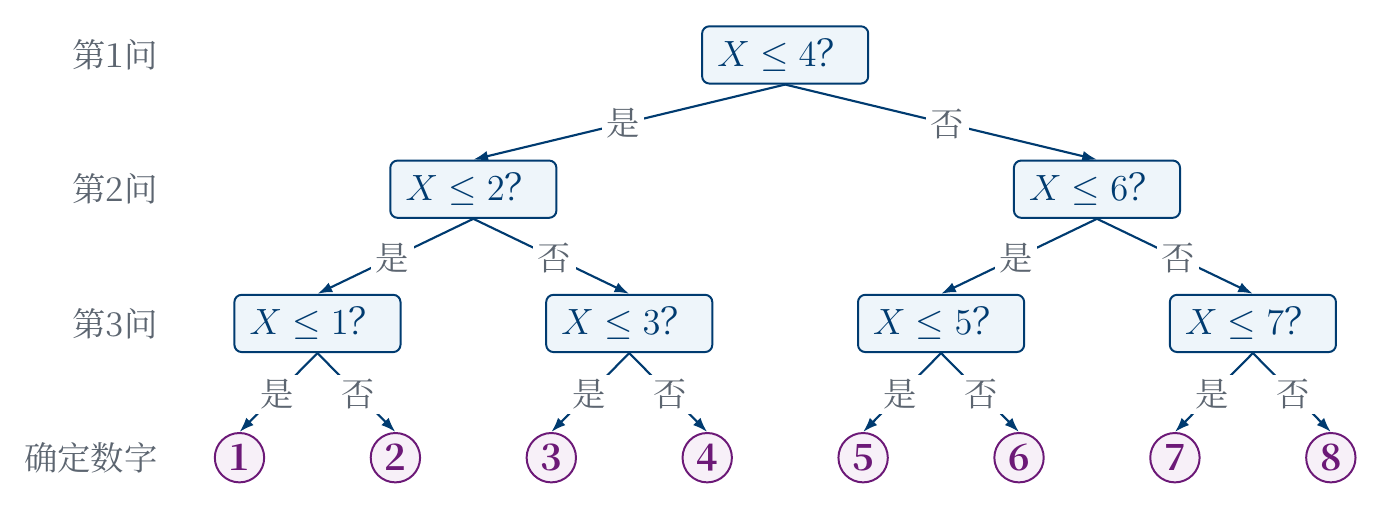
\includegraphics[width=0.9\linewidth]{tree1}
		\caption{Tree 1: Strategy 1}
		\label{fig:tree1}
	\end{figure}
	\begin{figure}
		\centering
		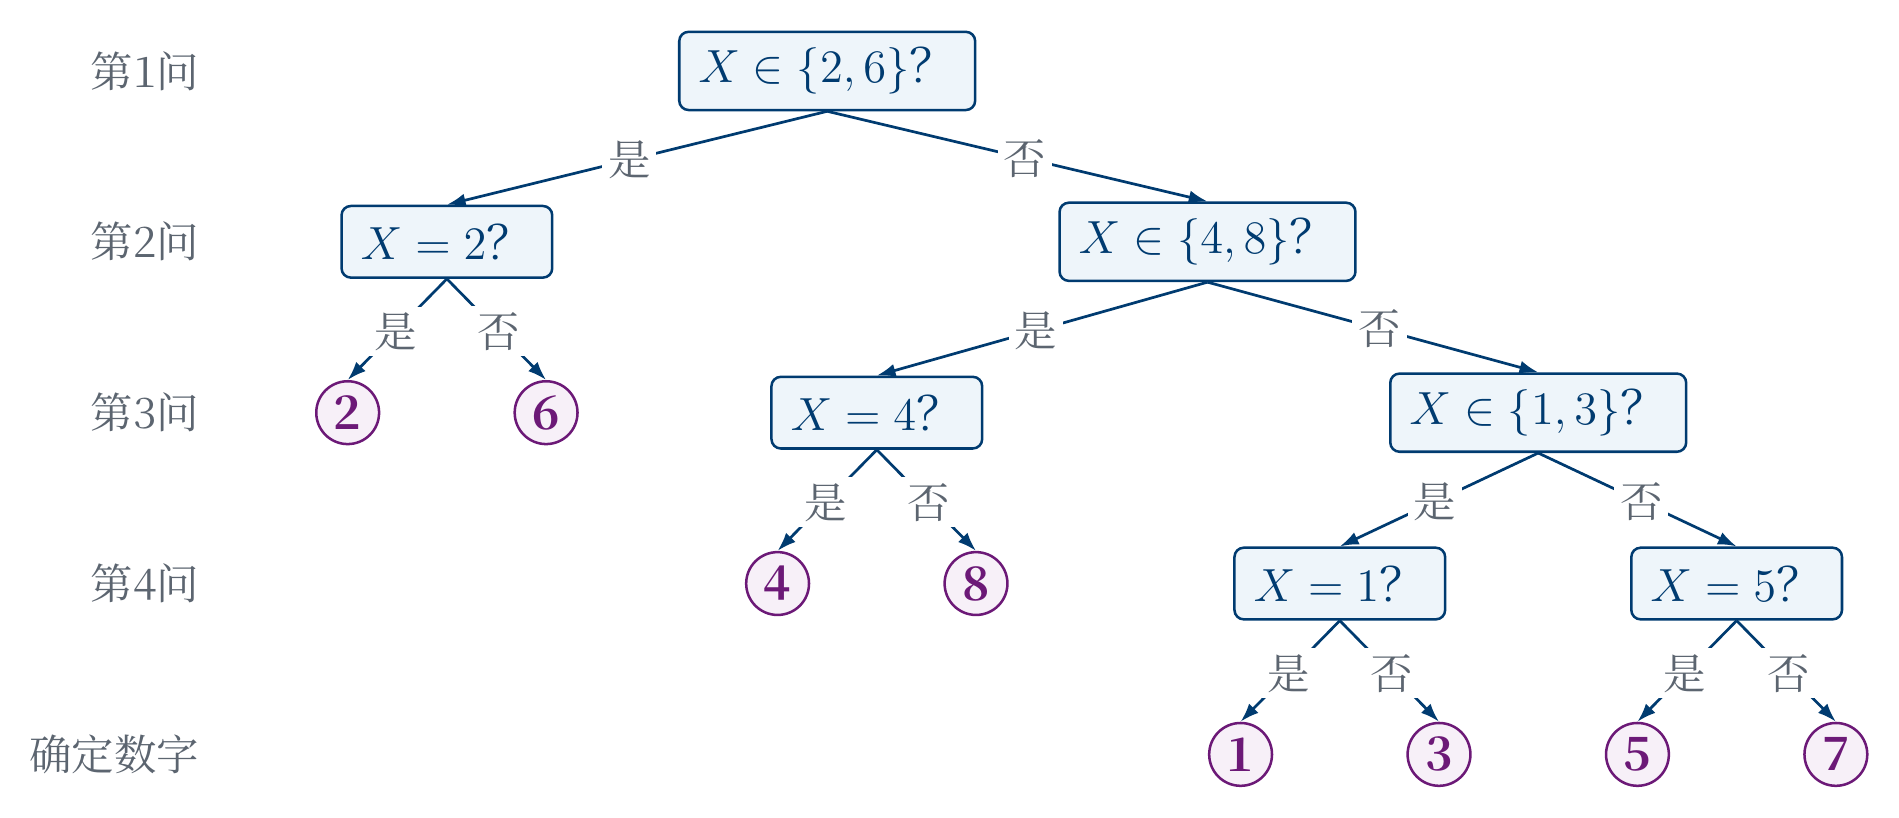
\includegraphics[width=0.9\linewidth]{tree2}
		\caption{Tree 2: Strategy 2}
		\label{fig:tree2}
	\end{figure}
	
	\subsection{Question 1}
	In the tree structure shown in \cref{fig:tree1}, each leaf node corresponding to Package A has a probability of $\frac{1}{8}$ of being reached, and the depth of each leaf node is 3. Therefore, the expected number of questions asked can be calculated as
	\[
	E(T_A)=3\times\frac{1}{8}\times8=3.
	\]
	
	For Package B, the probability of each leaf node is presented in \cref{tab:prob_yi}. Based on this distribution, the expected number of questions asked, $E(T_B)$, can be calculated as
	\[
	E(T_B) = 3\cdot\left(\frac{1}{16}\cdot4 + \frac{1}{4}\cdot2 + \frac{1}{8}\cdot2\right) = 3.
	\]
	
	\begin{table}[htbp]
		\centering
		\caption{Distribution of Package B}
		\label{tab:prob_yi}
		\begin{tabular}{lcccccccc}
			\toprule
			Leaf Node Depth \(i\) & 3 & 3 & 3 & 3 & 3 & 3 & 3 & 3 \\
			\midrule
			Probability \(P(X=i)\) & \(\frac{1}{16}\) & \(\frac{1}{4}\) & \(\frac{1}{16}\) & \(\frac{1}{8}\) & \(\frac{1}{16}\) & \(\frac{1}{4}\) & \(\frac{1}{16}\) & \(\frac{1}{8}\) \\
			\bottomrule
		\end{tabular}
	\end{table}
	
	\subsection{Question 2}
	In the tree structure shown in \cref{fig:tree2}, the expected number of questions asked under each package is presented in \cref{tab:Distribution of A and B}. The corresponding expectations can be calculated as follows:
	\[
	E(T_A) = \frac{1}{8} \times (2+2+3+3+4 \times 4) = \frac{13}{4} = 3.25 \\[10pt]
	\]
	\[
	E(T_B) = \frac{1}{4} \times 2 \times 2 + \frac{1}{8} \times 3 \times 2 + \frac{1}{16} \times 4 \times 4 = 2.75.
	\]
	
	\begin{table}[htbp]
		\centering
		\renewcommand{\arraystretch}{1.2}
		\caption{Tree 2: Strategy 2}
		\label{tab:Distribution of A and B}
		\begin{tabular}{ccccccccc}
			\toprule
			& 2 & 6 & 4 & 8 & 1 & 3 & 5 & 7 \\
			\midrule
			D & 2 & 2 & 3 & 3 & 4 & 4 & 4 & 4 \\
			A & \(\frac{1}{8}\) & \(\frac{1}{8}\) & \(\frac{1}{8}\) & \(\frac{1}{8}\) & \(\frac{1}{8}\) & \(\frac{1}{8}\) & \(\frac{1}{8}\) & \(\frac{1}{8}\) \\
			B & \(\frac{1}{4}\) & \(\frac{1}{4}\) & \(\frac{1}{8}\) & \(\frac{1}{8}\) & \(\frac{1}{16}\) & \(\frac{1}{16}\) & \(\frac{1}{16}\) & \(\frac{1}{16}\) \\
			\bottomrule
		\end{tabular}
	\end{table}
	
	\subsection{Question 3}
	The difference between the expected values under the two strategies indicates that Strategy 2 is more efficient than Strategy 1 in terms of the expected number of questions required. However, \cref{fig:tree2} illustrates that the decision tree associated with Strategy 2 has an imbalanced structure, resulting in a greater variance in the number of questions asked. Specifically,
	\[
	Var(T_{Strategy 1})=0.0625 \ll Var(T_{Strategy 2})=0.625.
	\]
	The greater variance associated with Strategy 2 may contribute to instability in the estimation process.
	
	\subsection{Question 4}
	The answer to this question is ``Impossible''. From the perspective of information theory, each question provides 1 bit of information. However, identifying the position of a number among eight possible positions requires 3 bits of information. This means that at least three questions must be asked on average.
	
\end{document}
